\documentclass[twoside,titlepage]{report}


\usepackage{amssymb,amsmath,amsfonts,amsthm,stmaryrd,fancyhdr,graphicx,color,multirow,pifont}
\usepackage[normalem]{ulem}
\usepackage{bigstrut}
\usepackage[all,cmtip]{xy}
\usepackage{microtype}

%% packages for the symbols activity:
%\usepackage{phaistos}
\usepackage{protosem}





%\usepackage{showkeys} %%% This package will show you your labels
                       %%% and should be commented out for the 
                       %%% final print out.
\usepackage{makeidx} %%% gives us our groovy index
%\usepackage[noDcommand]{kpfonts}

\makeindex

%\usepackage{layout} %%% Use command \layout in document to see margins
%%% Use package mathpazo to get another font

%%% These margins are set for 10 pt font size. 
%%% while some may find them to be too large, they 
%%% are set so that no more than 72 characters will
%%% be on any line.  This will help the readability 
%%% of the document.  If the font size is ever increased
%%% then the margins should be increased a bit too.
\oddsidemargin 62pt
\evensidemargin 62pt
\textwidth 345pt
\headheight 14pt




%%% Header and Footer Options
\renewcommand{\headrulewidth}{0.0pt} %%% this takes out the line 
%%%
%\rhead[]{\textsl{\leftmark}}  %%%
%\rfoot[]{\thepage}            %%% Options for 2 sided documents
%\lhead[\textsl{\rightmark}]{} %%%
%\lfoot[\thepage]{}            %%%
%%%
\lhead[\textsl{\rightmark}]{\textsl{\leftmark}} %%% Options for 1 sided documents
\cfoot[]{}                      %%% With typing on the *left* page
\rhead[]{}                                      %%% 
%%%
\cfoot[\thepage]{\thepage} %%% needed for both types of documents
%%% End Header and Footer Options


%%% This sets how the enumerate command works
\renewcommand{\theenumi}{$(\mathrm{\arabic{enumi}})$}
\renewcommand{\labelenumi}{\theenumi}
%\renewcommand{\topsep}{2em}
%%% This next bit of code defines all our theorem environments
\newtheoremstyle{SlantTheorem}{\topsep}{\topsep}%%% space between body and thm
		{\slshape}                      %%% Thm body font
		{}                              %%% Indent amount (empty = no indent)
		{\bfseries\sffamily}            %%% Thm head font
		{}                              %%% Punctuation after thm head
		{3ex}                           %%% Space after thm head
		{\thmname{#1}\thmnumber{ #2}\thmnote{ \bfseries(#3)}}%%% Thm head spec
\theoremstyle{SlantTheorem}
\newtheorem{thm}{Theorem}
\newtheorem*{para}{Paradox}
\newtheorem*{con}{Construction}
\newtheorem*{conj}{Conjecture}
\newtheorem{lem}[thm]{Lemma}
\newtheorem*{war}{WARNING}
\newtheorem*{eg}{Example}

\newtheoremstyle{problem}{\topsep}{\topsep}%%% space between body and thm
		{}                      %%% Thm body font
		{}                              %%% Indent amount (empty = no indent)
		{\bfseries}            %%% Thm head font
		{)}                    %%% Punctuation after thm head
		{ }                           %%% Space after thm head
		{\thmnumber{#2}\thmnote{ \bfseries (#3)}}%%% Thm head spec
\theoremstyle{problem}
\newtheorem{prob}{}[section]
\renewcommand{\theprob}{\arabic{prob}}

\newtheoremstyle{Definition}
{\topsep}{\topsep}{}{}{\sffamily\bfseries}{}{3ex}{}
\theoremstyle{Definition}
\newtheorem*{dfn}{Definition}

\newtheoremstyle{Exercises}
{\topsep}{\topsep}{}{}{\bfseries}{}{3ex}{}
\theoremstyle{Exercises}
\newtheorem*{ques}{Question}


\usepackage{array}
\setlength{\extrarowheight}{0cm}
\newdimen\digitwidth
\settowidth\digitwidth{9}
\def~{\hspace{\digitwidth}}
\def\divrule#1#2{
\noalign{\moveright#1\digitwidth
\vbox{\hrule width#2\digitwidth}}}



%%% This bit of code gives us our nice proof environment.
\renewenvironment{proof}[1][\proofname]{\begin{trivlist}\item[\hskip \labelsep \itshape \bfseries #1{}\hspace{2ex}]}
{\qed\end{trivlist}}
%%%

%%% This set of code gives us the unnumbered footnotes
\long\def\symbolfootnote[#1]#2{\begingroup\def\thefootnote{\fnsymbol{footnote}}
\footnote[#1]{#2}\endgroup}



%%% This set of code is all of our user defined commands
\newcommand{\bysame}{\mbox{\rule{3em}{.4pt}}\,}
\newcommand{\N}{\mathbb N}
\newcommand{\Z}{\mathbb Z}
\newcommand{\R}{\mathbb R}
\newcommand{\Q}{\mathbb Q}
\newcommand{\A}{\mathbb A}
\newcommand{\C}{\mathbb C}
\newcommand{\ph}{\varphi}
\newcommand{\ep}{\varepsilon}
\newcommand{\aph}{\alpha}
\newcommand{\QM}{\begin{center}{\huge\textbf{?}}\end{center}}
\renewcommand{\le}{\leqslant}
\renewcommand{\ge}{\geqslant}
\renewcommand{\a}{\wedge}
\renewcommand{\v}{\vee}
\renewcommand{\l}{\ell}
\renewcommand{\subset}{\subseteq}
\renewcommand{\supset}{\supseteq}
\renewcommand{\emptyset}{\varnothing}
\newcommand{\xto}{\xrightarrow}
\renewcommand{\qedsymbol}{$\blacksquare$}
\renewcommand{\bibname}{References and Further Reading}
\renewcommand{\abstractname}{Distributing this Document}
\renewcommand{\bar}{\protect\overline}
\renewcommand{\hat}{\protect\widehat}
\renewcommand{\tilde}{\widetilde}

\newcommand{\tri}{\triangle}

\newcommand{\mat}{\mathsf}
\renewcommand{\vec}{\overrightarrow}
\newcommand{\leftexp}[2]{{\vphantom{#2}}^{#1}{#2}}

\newcommand{\nocontentsline}[3]{}

\renewcommand*\thesection{\arabic{section}} % counts sections correctly


\begin{document}
\title{\textbf{\textsf{
\Huge History of Mathematics \\
\Large Math 2168: Spring 2014
}}}
\author{}
\date{}
\maketitle

%%%%
\cleardoublepage

\tableofcontents


\pagenumbering{arabic}
\pagestyle{fancy}
%%%%%%%%%%%%%%%%%%%%%%%%%%%%%%%%%%%%%%%%
%%%%%%% Sections to be included %%%%%%%%
%%%%%%%%%%%%%%%%%%%%%%%%%%%%%%%%%%%%%%%%

\renewcommand{\theenumi}{$(\mathrm{\alph{enumi}})$}
\renewcommand{\labelenumi}{\theenumi}

\newpage
\section{Food for Thought}	

Feel free to do these problems in any order.

\begin{prob}
What is a number? List out some qualities that you think a number has.
\end{prob}

\begin{prob}
How do you know when something is not a number?
\end{prob}

\begin{prob}
What are different ways we could represent numbers? 
\end{prob}

\begin{prob}
What if we used the following system:
\[
1 = a, \quad 2 = aa, \quad 3 = aaa, \quad\text{and so on.}
\]
What does the word \textit{concatenation} mean? How does it apply to
this system?  How would we add? How would we multiply? How could we
represent negative numbers?
\end{prob}


\begin{prob}
Once Oscar wondered what the number $\pi$ was. So he typed it into his
calculator and found:
\[
\pi = 3.1415926\dots
\]
Oscar then exclaimed, ``Ah now I know what number $\pi$ is.'' Can you
explain Oscar's thoughts on numbers?
\end{prob}


\newpage
\section{When in Rome\dots}

\begin{prob}
Count from 10--20 in the Hindu-Arabic, Roman, Mayan, Babylonian, and
Egyptian systems.
\end{prob}

\begin{prob}
Count from 100--200 \textit{by tens} in the Hindu-Arabic, Roman,
Mayan, Babylonian, and Egyptian systems.
\end{prob}

\begin{prob}
Count from 60--600 \textit{by sixties} in the Hindu-Arabic, Roman,
Mayan, Babylonian, and Egyptian systems.
\end{prob}

\begin{prob}
Discuss the advantages and disadvantages of the various systems. In
particular, can you distinguish between \textit{concatenation}
systems and \textit{place-value} systems?
\end{prob}

\begin{prob}
Adding and subtracting Roman numerals is perhaps easier than you may
think. For each of the problems above, give three examples of addition
problems using Roman numerals from the various ranges. See if you can
explain why Roman numerals were used in bookkeeping well into the
1700s. Big hint: Align like-letters when you can.
\end{prob}








\newpage
\section{Picture Yourself Dividing}


We want to understand how to visualize 
\[
\frac{a}{b} \div \frac{c}{d}
\]
Let's see if we can ease into this like a cold swimming pool.

\begin{prob}
Draw a picture that shows how to compute:
\[
6\div 3
\]
Explain how your picture could be redrawn for other similar numbers. 
\end{prob}

\begin{prob}
Try to use a similar process to the one you used in the first problem
to draw a picture that shows how to compute:
\[
\frac{1}{4} \div 3
\]
Explain how your picture could be redrawn for other similar numbers. 
\end{prob}


\begin{prob}
Try to use a similar process to the one you used in the first two problems
to draw a picture that shows how to compute:
\[
3 \div \frac{1}{4}
\]
Explain how your picture could be redrawn for other similar numbers. 
\end{prob}

\begin{prob}
Try to use a similar process to the one you used in the first three problems
to draw a picture that shows how to compute:
\[
\frac{5}{3} \div \frac{1}{4}
\]
Explain how your picture could be redrawn for other similar numbers.
\end{prob}

\begin{prob}
Explain how to draw pictures to visualize:
\[
\frac{a}{b} \div \frac{c}{d}
\]
\end{prob}

\begin{prob}
Use pictures to explain why:
\[
\frac{a}{b} \div \frac{c}{d} = \frac{a}{b} \cdot \frac{d}{c}
\]
\end{prob}


\newpage
\section{Friendly Pairs}

In this activity, we are going to play with pairs of numbers.  We'll
say that the pair $(a,b)$ is a ``friend'' to the pair $(c,d)$ if
$a\cdot d = b\cdot c$.

\begin{prob}
Give $5$ examples of pairs that are friends. Give $5$ examples of
pairs that are not friends.
\end{prob}

\begin{prob}\label{DF:2}
Is this a good rule?  That is, if $(a_1,b_1)$ is a friend to $(c,d)$
and $(a_2,b_2)$ is a friend to $(c,d)$, is it true that either
$(a_1,b_1)$ is a friend to $(a_2,b_2)$ or $(a_2,b_2)$ is a friend to
$(a_1,b_1)$?  If yes, justify your answer.  If no, give a
counterexample.
\end{prob}


Any counting number $a$ can be turned into a pair by the following
rule:
\[
a = (a,1)
\]

\begin{prob}\label{DF:3}
Suppose you can ``multiply'' pairs by the following rule:
\[
(a,b)\cdot (c,d) = (ac,bd)
\]
Is this a good rule, meaning do counting numbers still multiply the
correct way? Give three additional examples of pairs (that are not
integers) multiplying to make new pairs.
\end{prob}

\begin{prob}
Using the rules in Problem~\ref{DF:2} and Problem~\ref{DF:3} where now
the $a$, $b$, $c$, $d$, can themselves be pairs, simplify:
\[
\big((11,16),(3,5)\big)
\]
That is, show that $\big((11,16),(3,5)\big)$ is a friend to a simple
pair.
\end{prob}

\begin{prob}
What does any of this have to do with fractions? What does this have
to do with the ``invert and multiply'' rule for dividing fractions?
\end{prob}


\newpage
\section{Estimating the Area of a Circle}


Draw a (fairly large) circle on a blank sheet of paper. We'll think of
this as a unit circle.


\begin{prob}
Divide the unit circle into $2^2 = 4$ equal wedges each with its vertex at
the center of the circle $O$.  On each wedge, call the two corners of
the wedge that lie on the circle $A$ and $B_2$.  Let $\mathcal{A}_2$
denote the area of the triangle $\tri OAB_2$ and let $\theta_2$ denote the
measure of the angle at $O$. Explain how to estimate the area of the
circle with triangle $\tri OAB_2$. What is your estimate?
\end{prob}

\begin{prob}
Divide the unit circle into $2^3 = 8$ equal wedges each with its vertex at
the center of the circle $O$.  On each wedge, call the two corners of
the wedge that lie on the circle $A$ and $B_3$.  Let $\mathcal{A}_3$
denote the area of the triangle $\tri OAB_3$ and let $\theta_3$
denote the measure of the angle at $O$. Explain how to estimate the
area of the circle with triangle $\tri OAB_3$. What information do
you need to know to actually do this computation?
\end{prob}

\begin{prob}
Given an angle $\theta$, explain the relation of $\sin(\theta)$ and
$\cos(\theta)$ to the unit circle. How could these values help with
the calculation described above?
\end{prob}

\begin{prob}
Divide the unit circle into $2^n$ equal wedges each with its vertex at
the center of the circle $O$.  On each wedge, call the two corners of
the wedge that lie on the circle $A$ and $B_n$.  Let $\mathcal{A}_n$
denote the area of the triangle $\tri OAB_n$ and let $\theta_n$
denote the measure of the angle at $O$. Explain why someone would be
interested in the value of:
\[
\sin\left(\frac{\theta_n}{2}\right)
\]
\end{prob}

\begin{prob}
Recalling that:
\[
\sin\left(\frac{\theta}{2}\right) = \sqrt{\frac{1-\cos(\theta)}{2}}
\qquad\text{and}\qquad
\cos(\theta)^2 + \sin(\theta)^2 = 1
\]
Explain why:
\[
2 \mathcal{A}_{n+1} = \sqrt{\frac{1 - \sqrt{1 - (2\mathcal{A}_n)^2}}{2}}
\]
\end{prob}


\begin{prob} 
Let's fill out the following table (a calculator will help!):
\[
\begin{array}{| c || c | c | c | c | c |}
\hline\bigstrut
n  & \mathcal{A}_n & \text{Approx. Area} & \sqrt{1-(2\mathcal{A}_n)^2} & \frac{1 - \sqrt{1-(2\mathcal{A}_n)^2} }{2} &\rule[0mm]{0mm}{6mm}2\mathcal{A}_{n+1} =\sqrt{\frac{1 - \sqrt{1-(2\mathcal{A}_n)^2} }{2}} \\ \hline\hline 
2 &\rule[7mm]{20mm}{0mm}\hspace{20mm}  &\hspace{20mm}  &\hspace{20mm}  & \hspace{20mm} & \hspace{20mm}\\ \hline
3 &\rule[0mm]{0mm}{7mm}   &  &  & &   \\ \hline
4 &\rule[0mm]{0mm}{7mm}   &  &  & &   \\ \hline
5 &\rule[0mm]{0mm}{7mm}   &  &  & &   \\ \hline
6 &\rule[0mm]{0mm}{7mm}   &  &  & &   \\ \hline
7 &\rule[0mm]{0mm}{7mm}   &  &  & &   \\ \hline
8 &\rule[0mm]{0mm}{7mm}   &  &  & &   \\ \hline
\end{array}
\]
What do you notice?
\end{prob}


\newpage
\section{Euclid's Proof of Someone's Theorem}

\begin{prob}
Remind us, what is the most famous theorem of all and what exactly
does it assert?
\end{prob}

\begin{prob} 
What would one need to prove about the following diagram to prove the
``most famous theorem of all?''
\[
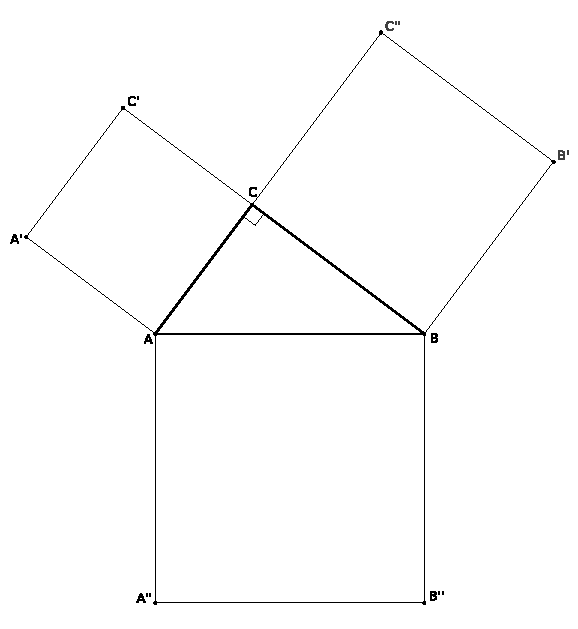
\includegraphics{../graphics/PythEuclid.pdf}
\]
\end{prob}

Let's see if we can do this!


\begin{prob}
Draw a line perpendicular to $\bar{AB}$ that passes though both $C$
and $\bar{A'' B''}$. Call the intersection between this line and
$\bar{AB}$, point $E$; call the intersection point between this line
and $\bar{A''B''}$, point $E'$. Explain why $\tri ACA''$ has half the
area of rectangle $AEE'A''$.
\end{prob}

\begin{prob}
Explain why $\tri ABA'$ has half the area of square $ACC'A'$.
\end{prob}

\begin{prob}
Explain why $\tri ACA''$ is congruent to $\tri ABA'$. 
\end{prob}

\begin{prob}
Explain why area of square $ACC'A'$ is equal to the area of rectangle
$AEE'A''$.
\end{prob}


\begin{prob}
Use similar ideas to complete a proof the ``most famous theorem of
all.''
\end{prob}




\newpage
\section{Of Course All Right Angles are Congruent\dots}	


\begin{prob}
Put a dot at the center of a blank sheet of paper and call it $O$.
Use a protractor to draw an angle of $50^\circ$ with vertex at the
point $O$ and sides extending all the way out to the edge of the
paper.  Cut the paper along one side of the angle and one side only.
Make a cone by moving the cut edge to the other side of the angle you
drew.  This cone (extended infinitely) is your universe.
\end{prob}


\begin{prob}
Does Euclid's 1st Postulate hold in your universe? Explain your reasoning.
\end{prob}

\begin{prob}
Does Euclid's 2nd Postulate hold in your universe? Explain your reasoning.
\end{prob}

\begin{prob}
Does Euclid's 3rd Postulate hold in your universe? Explain your reasoning.
\end{prob}

\begin{prob}
You measure angles on your universe by laying the paper out flat and
measuring the angles on the paper. Draw a line that passes through $O$
along the cut edge. Now lay your paper flat and bisect the angle
formed by the other edge and your line. What does this say about
Euclid's 4th Postulate? Explain your reasoning.
\end{prob}



\begin{prob}
Does Euclid's 5th Postulate hold in your universe? Explain your
reasoning. Big hint, how few sides can a $n$-gon have?
\end{prob}


\newpage
\section{Triangles on a Cone}	


\begin{prob}
Put a dot at the center of a blank sheet of paper and call it $O$.
Use a protractor to draw an angle of $50^\circ$ with vertex at the
point $O$ and sides extending all the way out to the edge of the
paper.  Cut the paper along one side of the angle and one side only.
Make a cone by moving the cut edge to the other side of the angle you
drew.  This cone (extended infinitely) is your universe.
\end{prob}


\begin{prob}
Make a triangle in your universe that surrounds $O$. To do this,
unfold your universe and lay it out flat on the desk and make the
sides with your ruler.  When a side gets to the cut side of your
angle, put the other side of the angle on top and keep going.
\end{prob}

\begin{prob}
You measure angles on your universe by laying the paper out flat and
measuring the angles on the paper. Measure the angles in your
triangle, what do they sum to?
\end{prob}


\begin{prob}
Repeat the problems above, but this time cut an angle of $40^\circ$ to
make your cone. What do you notice?
\end{prob}

Let's see if we can explain this. Do you know who is eager to help
you? That's right: Louie Llama.
\[
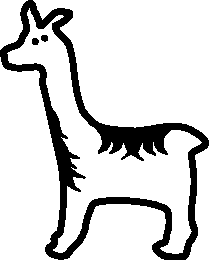
\includegraphics[height=1in]{../graphics/llama.pdf}
\]

\begin{prob}
Take your triangle and denote the measure of its angles as $a$, $b$,
and $c$. We would like to parade Louie around the triangle. There is
only one catch: What happens to Louie when he passes over the ``cut?''
Draw some pictures and see if you can figure it out.
\end{prob}

Start Louie Llama out along a side adjacent to the angle of measure
$a$. He should be on the outside of the triangle, his feet should be
pointing toward the triangle, and his face should be pointing toward
the angle of measure $b$. Continue this process and walk him all
around the triangle. When he gets to the ``cut'' put the paper
together, and let him continue his walk.

\begin{prob} 
Through what angle does Louie rotate when he strolls around a vertex?
\end{prob}

\begin{prob}
How many degrees did the ``cut'' rotate Louie? 
\end{prob}

\begin{prob} 
All in all, how many degrees did Louie Llama rotate in his walk?
\end{prob}


\begin{prob}
If a cone is made on a sheet of paper with a cut of $\theta$ degrees,
and a triangle is made surrounding the point of the cone, what is the
sum of the degrees of this triangle?
\end{prob}




\begin{prob}
Explain why not all of Euclid's postulates could hold in this
universe. Exactly which postulates don't hold?
\end{prob}


\newpage
\section{Classy Work}	


\begin{prob} 
What is a regular tessellation? Classify all regular tessellations and
explain how you know you have found all of them.
\end{prob}


\begin{prob}
What is a Platonic solid? Classify all Platonic solids and
explain how you know you have found all of them.
\end{prob}

\begin{prob}
What is the connection between the first two questions?
\end{prob}


\begin{prob}
Build the Platonic solids.
\end{prob}

\begin{prob}
Take two tetrahedrons. Glue them together along one of the triangular
faces. Is this a \textit{sixth} Platonic solid? Explain your
reasoning.
\end{prob}




\newpage
\section{Polyhedral Planets}	


In this activity, we will suppose in turn that you live on a planet
that is shaped like each of the regular convex polyhedra---not unlike
\textit{Le Petit Prince} who lives on an asteroid.

\begin{prob}
Considering each of the five regular convex polyhedra in turn, what
fraction of the planet's surface could you see if you stood:
\begin{enumerate}
\item In the middle of a face? 
\item In the middle of an edge?
\item On a vertex?
\end{enumerate}
In each case, explain your reasoning.
\end{prob}



\begin{prob}
Now suppose that you wish to go on a walk, surveying your polyhedral
planet. For each platonic solid, give the shortest path you can (draw
it on a net) that would allow you to observe the entire planet. In
each case, explain your reasoning.
\end{prob}


\newpage
\section{Symmetry is the Key}	

It is believed by some physicists that the fundamental forces of the
universe are related via symmetry. In this activity, we will see how
the symmetries of even the simplest 3D solid are in fact quite
complex. \textbf{You'll need a real-life tetrahedron for this
activity.}



\begin{prob}
Make a group table of all the rotational symmetries of your
tetrahedron.
\[
\begin{array}{|c||c|c|c|c|c|c|c|c|c|c|c|c|}
\hline
\circ & \rule[7mm]{7mm}{0mm} & \rule[7mm]{7mm}{0mm}  &\rule[7mm]{7mm}{0mm}  &\rule[7mm]{7mm}{0mm} &\rule[7mm]{7mm}{0mm} &\rule[7mm]{7mm}{0mm} &\rule[7mm]{7mm}{0mm} &\rule[7mm]{7mm}{0mm} &\rule[7mm]{7mm}{0mm} &\rule[7mm]{7mm}{0mm} &\rule[7mm]{7mm}{0mm} &\rule[7mm]{7mm}{0mm} \\ \hline\hline
\rule[7mm]{7mm}{0mm} & & & & & & & & & & & & \\ \hline
\rule[7mm]{7mm}{0mm} & & & & & & & & & & & & \\ \hline
\rule[7mm]{7mm}{0mm} & & & & & & & & & & & & \\ \hline
\rule[7mm]{7mm}{0mm} & & & & & & & & & & & & \\ \hline
\rule[7mm]{7mm}{0mm} & & & & & & & & & & & & \\ \hline
\rule[7mm]{7mm}{0mm} & & & & & & & & & & & & \\ \hline
\rule[7mm]{7mm}{0mm} & & & & & & & & & & & & \\ \hline
\rule[7mm]{7mm}{0mm} & & & & & & & & & & & & \\ \hline
\rule[7mm]{7mm}{0mm} & & & & & & & & & & & & \\ \hline
\rule[7mm]{7mm}{0mm} & & & & & & & & & & & & \\ \hline
\rule[7mm]{7mm}{0mm} & & & & & & & & & & & & \\ \hline
\rule[7mm]{7mm}{0mm} & & & & & & & & & & & & \\ \hline
\end{array}
\]

\end{prob}

\begin{prob}
Is the group commutative?
\end{prob}

\begin{prob}
What elements of the group commute with all other elements? Do they
themselves form a group?
\end{prob}

\begin{prob}
Can you find a subgroup containing exactly $n$ elements when
$n=2,3,4,5,\dots,12$? Which integers work and which don't?
\end{prob}



\newpage
\section{Owing Numbers}	

You are an Indian mathematician back in the year 650 working with
Brahmagupta and Bhaskara.  You know only the counting numbers and 0.
You learned in school how to add and multiply in this number system.

commutative. 

\begin{prob}
In school you learned:
\begin{itemize}
\item Both addition and multiplication were
associative and commutative. Explain what this means.
\item The number $0$ is an identity element for addition and 1 is an
identity element for multiplication. Explain what this means.
\item The distributive law holds.  Explain what this means.
\item The cancellation property holds, meaning:
\begin{align*}
a + b &= a + c  & a \cdot b &= a \cdot c\\
&\Rightarrow b = c & &\Rightarrow{b = c}
\end{align*}
Give examples of the cancellation properties. 
\end{itemize}
\end{prob}

\begin{prob}
Suppose there were some new numbers $e$ and $f$ such that
\[
e+ n = n\qquad\text{and}\qquad f\cdot n = n
\]
for every counting number $n$. Explain why $e$ must in fact be equal to
$0$ and $f$ must be in fact equal to $1$.
\end{prob}


\begin{prob}
Explain why given any counting number  $n$
\[
0 \cdot n = 0
\]
Big hint: Use the fact that $0 + 0 = 0$.
\end{prob}

You think the number system should be enlarged to
incorporate \textit{owing} an amount as well as \textit{having} an
amount. That's easy, just adjoin the numbers
$\{\tilde{1}, \tilde{2},\dots\}$.  Adding in this bigger number
system, that you call the integers, is easy, and you still have that
addition is associative and commutative, and that $0$ is still the
identity element for addition.  Defining multiplication of two numbers
$a\cdot b$ is not so easy when at least one of the two numbers is
negative.  You want to define it so that multiplication is still
associative and commutative, that $1$ is still the identity for
multiplication, and so that the distributive law continues to hold.


\begin{prob}
Explain why 
\[
m\cdot\tilde{n} = \tilde{m\cdot n}
\]
 where $m$ and $n$ are counting numbers (or $0$)?
\end{prob}


\begin{prob}
Use the problem above to explain why this forces you to define
\[
\tilde{m}\cdot \tilde{n} = m\cdot n 
\]
when $m$ and $n$ are counting numbers (or $0$)?
\end{prob}

\begin{prob}
What facts about negative numbers are we illustrating?
\end{prob}


\newpage
\section{Trigonometry Before Sine and Cosine}	

In this activity, we are going to explore how someone could \textit{understand} that 
\begin{align*}
\sin\left(\frac{\theta}{2}\right) &= \sqrt{\frac{1-\cos(\theta)}{2}}\\
&=\sqrt{\frac{1 - \sqrt{1 - \sin(\theta)^2}}{2}},
\end{align*}
\textit{before} we had the notions of sine and cosine. Consider the following unit circle:
\[
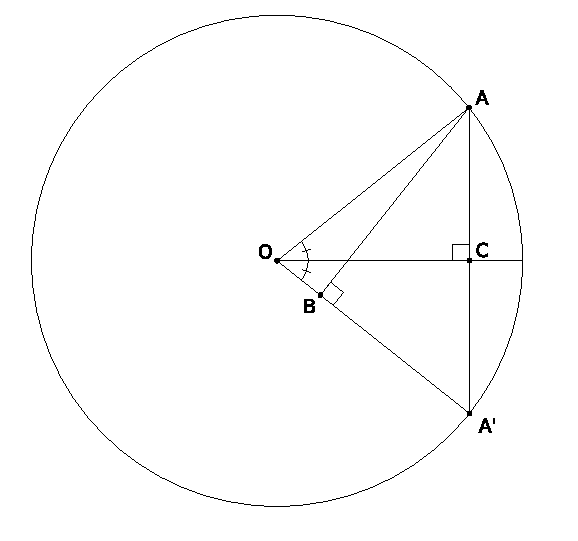
\includegraphics{../graphics/HalfAngleFormula.pdf}
\]


\begin{prob} 
Explain why $\tri OCA$ is similar to $\tri ABA'$.
\end{prob}

\begin{prob} 
Explain why $|BA'| = |CA|\cdot |AA'| = 2|CA|^2$.
\end{prob}

\begin{prob} 
Explain why $|OB|^2 = (1-2|CA|^2)^2$.
\end{prob}

\begin{prob} 
Explain why $|BA|^2 = 1-(1-2|CA|^2)^2$.
\end{prob}


\begin{prob} Solve for $|CA|$ in terms of $|BA|$.
\end{prob}

\begin{prob}
Explain how we have done what we set out to do.
\end{prob}


\newpage
\section{Geometry and Quadratic Equations}	



In ancient and Medieval times the discussion of quadratic equations
was often broken into three cases:
\begin{enumerate}
\item $x^2 + bx = c$
\item $x^2 = bx + c$
\item $x^2 + c = bx$
\end{enumerate}
where $b$ and $c$ are positive numbers. 


\begin{prob}
Create real-world word problems involving length and area for each
case above.
\end{prob}

\begin{prob}
Solve each of the three cases above by actually ``completing the
square'' using a \textbf{real} square.
\end{prob}

\begin{prob}
Is this a complete list of cases? If not, what is missing and why is
it (are they) missing? Explain your reasoning.
\end{prob}





\newpage
\section{State of the Art Circa 1550}	

Somewhere deep in your brain is a sleeping technique\dots AWAKE!
We want to solve:
\[
x^3 + 9x -26 =0
\]
We're going to have to use the Ferro-Tartaglia method, but all I can tell you are these three steps:
\begin{enumerate}
\item Replace $x$ with $u+v$. 
\item Set $uv$ so that all of the terms are eliminated except for $u^3$,
$v^3$, and constant terms.  
\item Clear denominators and use the quadratic formula.
\end{enumerate}


\begin{prob}
Use the Ferro-Tartaglia method to solve $x^3 + 9x -26 =0$.
\end{prob}


\begin{prob}
How many solutions should our equation above have? Where/what are they?
Hint: Make use of an old forgotten foe\dots
\end{prob}


\newpage
\section{A Whole New World}	

\begin{prob}
List Euclid's five postulates. Draw pictures representing these
postulates.
\end{prob}

\begin{prob}
Here are other statements closely related to Euclid's fifth postulate:
\begin{enumerate}
\item[(5A)] Exactly one line can be drawn through any point not on a given line parallel to the given line. 
\item[(5B)] The sum of the interior angles of every triangle is equal to $180^\circ$.
\item[(5C)] If two lines $\l_1$ and $\l_2$ are both perpendicular to some third line, then 
$\l_1$ and $\l_2$ do not meet.
\end{enumerate}
draw pictures depicting these statements.  Can you explain why
Euclid's fifth postulate is sometimes called the \emph{parallel
postulate}?
\end{prob}

There is a very natural geometry where the sum of the angles in every
triangle is \textit{greater than} $180^\circ$ and the essences of the
first four also still hold. Instead of working with a plane, we now
work on a sphere. We call this sort of geometry
\textit{Spherical Geometry}. Points, circles, angles, and
distances are exactly what we would expect them to be. But what do we
mean by lines on a sphere?  Lines are supposed to be extended
indefinitely.  In Spherical Geometry, the lines are the \emph{great
circles}. 

\begin{dfn}
A \textbf{great circle} is a circle on the sphere with the same center
as the sphere.
\end{dfn}

\begin{prob}
Draw some pictures of great circles and see if you can explain what
the definition above is saying.
\end{prob}

It is a theorem of Euclidean Geometry that the shortest path between
any two points on a plane is given by a line segment. We have a
similar theorem in Spherical Geometry.
\begin{thm}
The shortest path between any two points on a sphere is given by an
arc of a great circle.
\end{thm}


\begin{prob}
In Spherical Geometry, what is the difference between a great circle
and a regular Spherical Geometry circle?  Try to come up with a
definition of a \textit{circle} that will be true in both Euclidean
and Spherical Geometry.
\end{prob}

\begin{prob} Explain why the following proposition from Euclidean Geometry
  does not hold in Spherical Geometry: A triangle has at most one
  right angle.  (Can you find a triangle in Spherical Geometry with
  three right angles?)
\end{prob}

\begin{prob}
Explain why the following result from Euclidean Geometry does not hold
in Spherical Geometry: When the radius of a circle increases, its
circumference also increases.
\end{prob}

\begin{prob}
Define distinct lines to be \textbf{parallel} if they do not
intersect. Can you have parallel lines in Spherical Geometry?  Explain
why or why not.
\end{prob}


\begin{prob}
Come up with a definition of a \textit{polygon} that will be
true in both Euclidean and Spherical Geometry.
\end{prob}


\begin{prob}
A mathematician goes camping. She leaves her tent, walks one mile due
south, then one mile due east. She then sees a bear before walking one
mile north back to her tent. What color was the bear?
\end{prob}

\begin{prob}
The great German mathematician Gauss measured the angles of the
  triangle formed by the mountain peaks of Hohenhagen, Inselberg, and
  Brocken. What reasons might one have for doing this?
\end{prob}


\newpage
\section{Disk World}	


Once humans became comfortable with Euclidean Geometry, we took the
next step: Could the postulates and proofs be improved? In particular,
the Parallel Postulate seemed overly complicated. Could it
be \textit{proven} from the previous four, or was it really necessary?
It was not until the early 19th century that the mystery about the
role of the Parallel Postulate was solved and its absolute necessity
was shown. This was done by constructing geometries in which all of
Euclid's other postulates are true but the Parallel Postulate
is \textbf{false}.  Here is a construction that depends on two things:
\begin{enumerate}
\item Algebraic formulas about the distances between points on a circle. 
\item A geometric construction.
\end{enumerate}

Start with a circle of radius of $5$ cm, center $O$ and two points $A$
and $B$ inside it---place $A$ and $B$ near the edges.  The inside of
this circle will be called the \textbf{hyperbolic plane}.

\begin{prob} 
Use a ruler and calculator to calculate:
\[
\frac{5^2}{|OA|}.
\]
\end{prob}

\begin{prob} 
Extend the ray $\vec{OA}$ far enough outside the circle to be able to mark the point $A'$ such that
\[
|OA'| = \frac{5^2}{|OA|}.
\]
\end{prob}

\begin{prob}
Construct the circle passing through $A$, $A'$, and $B$.  Call the two
points where our two circles intersect $P$ and $Q$. 
\end{prob}

The points $P$ and $Q$ divide the newly constructed circle into two
arcs, the arc inside the hyperbolic plane and the arc outside the
hyperbolic plane.  Call the inside arc the \textbf{hyperbolic line}
passing through $A$ and $B$.

We need to have notions of \textit{distance} and \textit{angle} to
have a geometry.  The \textbf{angle} between two hyperbolic lines that
cross at a point $X$ is just the angle between the tangent lines to
the two pieces of circle. The \textbf{hyperbolic distance} between two
points, for example the two points $A$ and $B$ we started with, is
found via some complicated algebra:
\[
d_H(A,B) = \left|\ln\left(\frac{|AP|}{|BP|} \cdot \frac{|BQ|}{|AQ|} \right)\right|
\]

\begin{prob}
Does $d_H(A,B) = d_H(B,A)$?
\end{prob}

\begin{prob}
What happens to $d_H(A,B)$ when $A$ is fixed and $B$ gets closer and
closer to the edge of the circle?
\end{prob}

\begin{prob}
If $A$, $B$, and $C$ are on the same hyperbolic line, with $B$ between
$A$ and $C$, can you explain why $d_H(A,C) = d_H(A,B)+ d_H(B,C)$?
\end{prob}


\newpage
\section{Projective Geometry}

While people were still struggling with Euclid's postulate (until the
19th Century) the Renaissance was happening in Europe (15th Century).
In Italy this brought with it an interest in exploration and realism
in painting.  Realism demanded the understanding of perspective, that
is, how to faithfully represent the eye's view of a (3-dimensional)
landscape or other object extending off into the distance (two rails
of a train-track converging in the distance---small problem: There
were no railroads during the Renaissance).  Logical conclusion: There should
be a point infinitely far away where the two (parallel) rails meet.
In fact the geometers made those infinitely far away points.  Let's
see how.

The solid lines are the axes of 3-dimensional Euclidean space with
origin $O$.  The dotted plane is our canvas.
\[
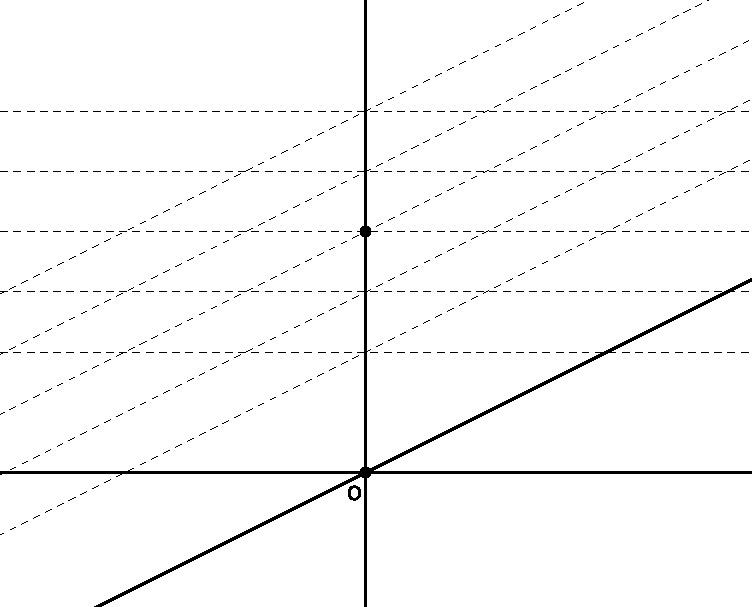
\includegraphics{../graphics/projPlane.pdf}
\]


\begin{prob} 
Put a point $A$ on the canvas.  Draw the line through $O$ and $A$ (and
extend it infinitely in both directions).
\end{prob}

\begin{prob} 
Put a point $B$ on the canvas.  Draw the line through $O$ and $B$ (and
extend it infinitely in both directions).
\end{prob}

\begin{prob} 
Does each point on the canvas determine a line through $O$?  Do
different points determine different lines through $O$?
\end{prob}

\begin{prob}\label{P:Start} 
Are there some lines through $O$ that get missed, that is, lines that
don't correspond to points on the canvas? Which ones?  We will say
that each of those lines corresponds to a `canvas point at infinity.'
\end{prob}

\begin{prob} 
Draw some train tracks (parallel lines $l$ and $m$) on the canvas.  Show
that each rail (line) determines a plane through $O$.
\end{prob}

\begin{prob}\label{P:Finish}
Let $L$ and $M$ stand for the planes through $O$ corresponding to the lines
$l$ and $m$ respectively.  How do $L$ and $M$ intersect?
\end{prob}

\begin{prob}
How do you find the line at which the planes $L$ and $M$ intersect?
\end{prob}

\begin{prob} 
Why do Problems \ref{P:Start} through \ref{P:Finish} above justify the
statement that ``parallel lines on the canvas also meet at exactly one
point, it's just that point is a canvas point at infinity?''
\end{prob}






\newpage
\section{Coordinate Geometry}


Mathematicians in Europe in the 17th Century were just beginning to
come to terms with representing algebraic relations geometrically
using a coordinate plane, and conversely, representing geometric loci
in the (coordinate) plane by algebraic relations.  The solution to
solving this problem for one particular kind of locus was to have
spectacular consequences in astronomy and physics within a century,
and was all tied up with the discovery of calculus by Newton and
Leibniz.

In this activity we will explore the locus of points $(x,y)$ such that
the distance between $(x,y)$ and $(5,0)$ plus the the distance between
$(x,y)$ and $(-4,0)$ is equal to $15$.
\[
%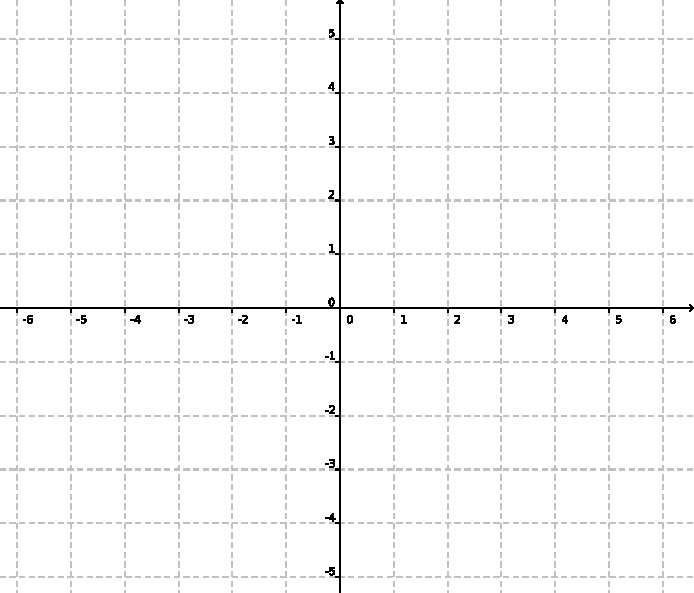
\includegraphics{../graphics/coordPlane.pdf}
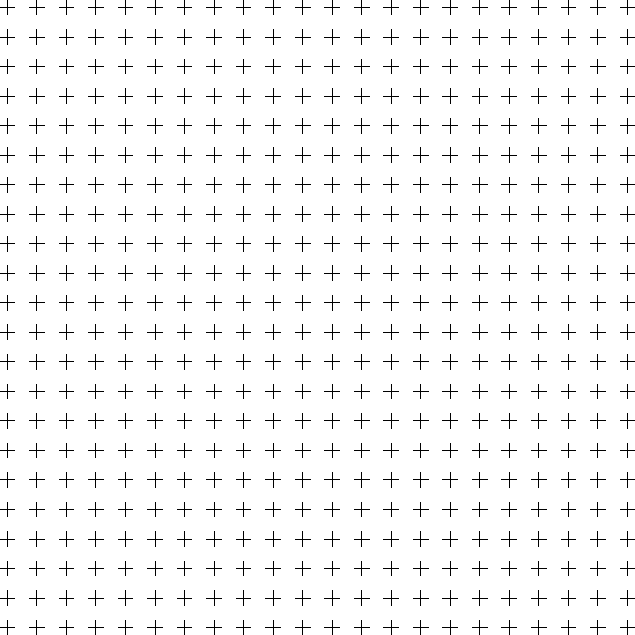
\includegraphics{../graphics/complexPlane.pdf}
\]

\begin{prob}
Pick two points, one inside your locus and another outside.
\end{prob}


\begin{prob}
Find four points that are exactly on the locus.  Hint: You can do two
in your head, but you may need the Pythagorean theorem and the
quadratic formula to get the other two.
\end{prob}

\begin{prob} 
Write ``the distance between $(x,y)$ and $(5,0)$ plus the the distance
between $(x,y)$ and $(-4,0)$ is equal to $15$'' as an algebraic
equation.
\end{prob}

Now we will attempt to put the equation above into ``standard form:''
\[
\frac{(x-h)^2}{a^2} + \frac{(y-k)^2}{b^2} = 1
\]

\begin{prob}
To start, isolate one of the square-roots, and square both sides.
\end{prob}

\begin{prob}
Next, isolate the other square-root, and square both sides. 
\end{prob}

\begin{prob}
Complete the square, and get it into standard form! Can you figure out what $a$, $b$, $h$, and $k$ represent?
\end{prob}



\newpage
\section{Complex Numbers From Different Angles}


In this activity we will investigate complex multiplication.

\begin{prob} Consider the innocent little equation:
\[
x^3 -1 = 0
\]
How many solutions does it have? What are they? Plot them on the
complex plane below.
\[
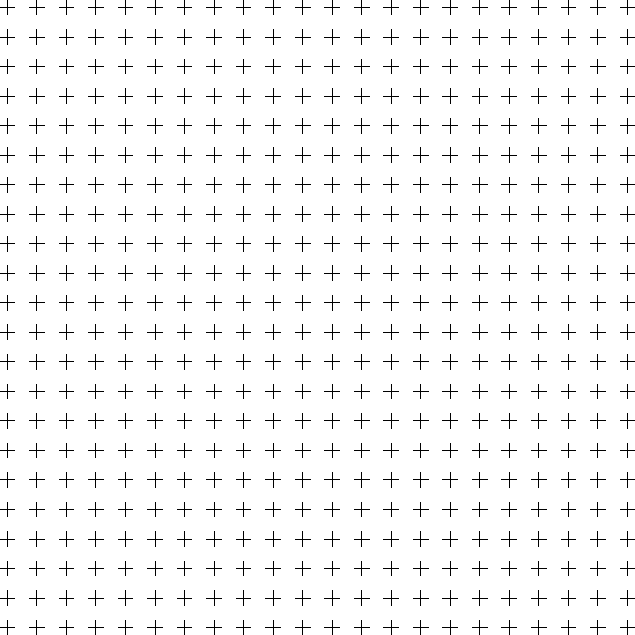
\includegraphics{../graphics/complexPlane.pdf}
\]
\end{prob}

\begin{prob}
Thinking about your work above, see if you can solve:
\[
x^4 -1 = 0
\]
Plot the solutions on the complex plane below.
\[
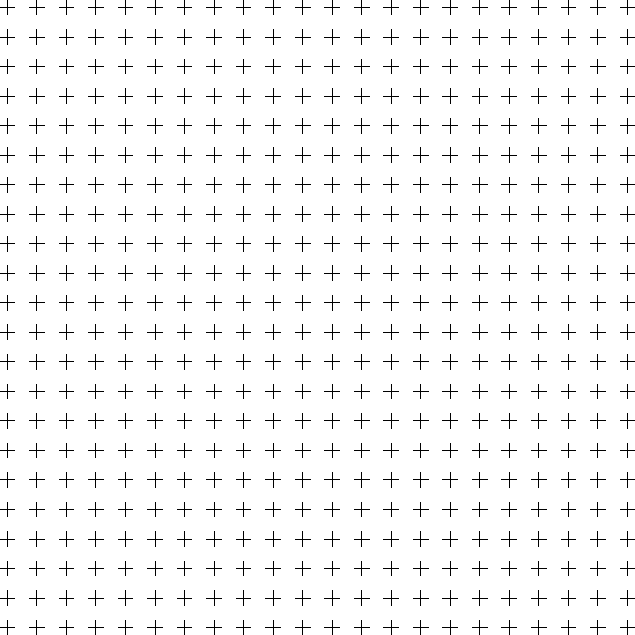
\includegraphics{../graphics/complexPlane.pdf}
\]
\end{prob}


\begin{prob}
Suppose I told you that:
\begin{align*}
\sin(x) &= x - \frac{x^3}{3!} + \frac{x^5}{5!} - \frac{x^7}{7!} + \dots + \frac{(-1)^n x^{2n+1}}{(2n+1)!} + \cdots \\
\cos(x) &= 1 - \frac{x^2}{2!} + \frac{x^4}{4!} - \frac{x^6}{6!} + \dots + \frac{(-1)^n x^{2n}}{(2n)!} + \cdots \\
e^x &= 1 + x + \frac{x^2}{2!} + \frac{x^3}{3!} + \frac{x^4}{4!} + \dots + \frac{x^n}{n!} + \cdots 
\end{align*}
Explain why we say:
\[
e^{x\cdot i} = \cos(x) + i \sin(x)
\]
\end{prob}

\begin{prob}
 This is Euler's famous formula:
\[
e^{\pi \cdot i } + 1 = 0
\]
Use the problem above to explain why it is true.
\end{prob}

\begin{prob}
What does all this have to do with De Moivre's Theorem?
\end{prob}

\begin{prob}
How can you use this to take the $n$th root of a complex number?
\end{prob}


\newpage
\section{De Moivre Saves the Day!}

The rules for solving second and third degree equations led to a
``sticky wicket.''  Namely the rule for solving a quadratic equation
forced its user to take the square root of a number that was sometimes
negative.  Worse yet, the formula for solving a cubic equation forced
the user to take the cube root of a number that resulted from taking
square roots!  Despite misgivings, mathematicians were eventually
forced to expand the number system to one where square roots can be
found for any of its numbers.

You may recall that the Ferro-Tartaglia method gives 
\[
\sqrt[3]{\frac{-1+\sqrt{-31}}{2}} + \frac{2}{\sqrt[3]{\frac{1}{2}(-1+\sqrt{-31})}}
\]
as a solution to: $y = x^3-6x+1$. Moreover, as this plot of $y = x^3-6x+1$ shows
\[
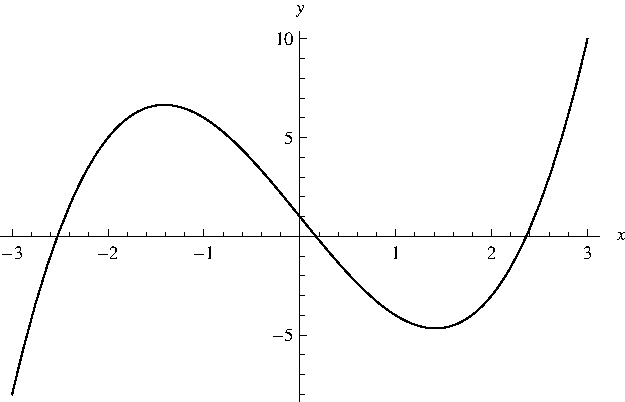
\includegraphics[width=3in]{../graphics/cubicPlot.pdf}
\]
this must be a real solution\dots But how? There is a square-root of a
negative number in the expression above! 

We're going to investiagate incredible connection between adding and
multiplying complex numbers and plane geometry.  It's called \textit{De
Moivre's rule}---it is here to save the day.  Please fasten your seat
belts and place your trays in the upright position.



You will need a scientific calculator and a straight-edge and compass.

\break

\begin{prob}
Plot the point $(4,3)$ in the plane below---let each square be $1/2$
unit.  We will think of this point as the complex number $4 + 3i$.
\[
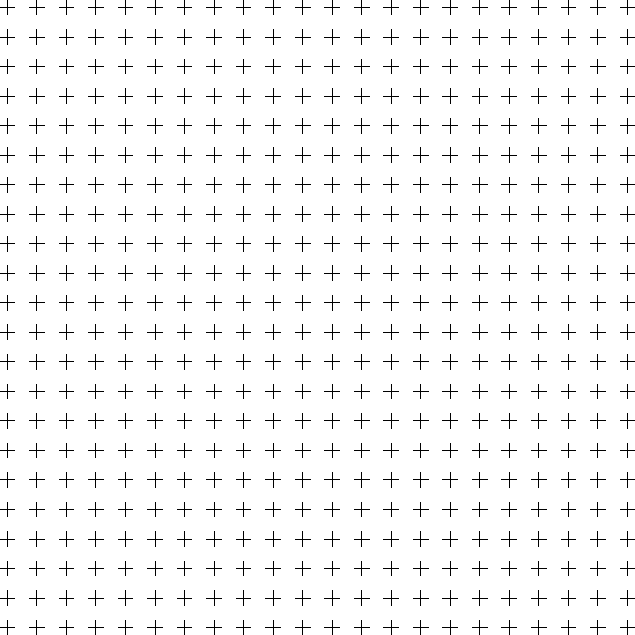
\includegraphics{../graphics/complexPlane.pdf}
\]
\begin{enumerate}
\item Draw the ray from the origin through your chosen complex number.
\item Measure its distance to the origin (called the \textit{absolute value} of the complex number $4 + 3i$). 
\item Use inverse tangent to measure the angle between your complex number and the positive real axis. 
\end{enumerate}
\end{prob}

\begin{prob}
We're going to solve $(x+yi)^3 = 4+3i$ for $x$ and $y$ using geometry!
\begin{enumerate}
\item Compute the cube root of the absolute value you found before. 
\item Compute one-third of the angle you found before. 
\item Use sine and cosine to finish it off!
\item How can you check your work? Do it.
\end{enumerate}
\end{prob}


\begin{prob}
Now use De Moivre's method to take the cube roots found in:
\[
\sqrt[3]{\frac{-1+\sqrt{-31}}{2}} + \frac{2}{\sqrt[3]{\frac{1}{2}(-1+\sqrt{-31})}}
\]
\end{prob}


%\newpage
\section{Attack of Ferro-Tartaglia}

You may recall that the Ferro-Tartaglia method gives 
\[
\sqrt[3]{\frac{-1+\sqrt{-31}}{2}} + \frac{2}{\sqrt[3]{\frac{1}{2}(-1+\sqrt{-31})}}
\]
as a solution to: $y = x^3-6x+1$. Moreover, as this plot of $y = x^3-6x+1$ shows
\[
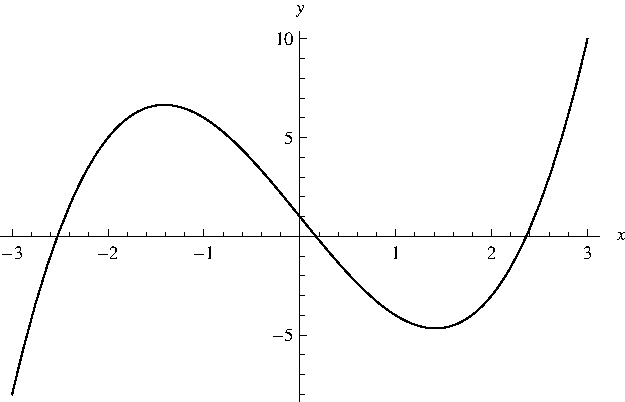
\includegraphics[width=3in]{../graphics/cubicPlot.pdf}
\]
this must be a real solution\dots But how? There is a square-root of a
negative number in the expression above! Ok, uncharacteristically for
me, I'll show you how this is done. Please fasten your seat belts and
place your trays in the upright position.

Start by looking at:
\[
\frac{-1+\sqrt{-31}}{2} = \frac{-1}{2} + \frac{\sqrt{31}}{2} i 
\]
If we plot this in the complex plane, we get:
\[
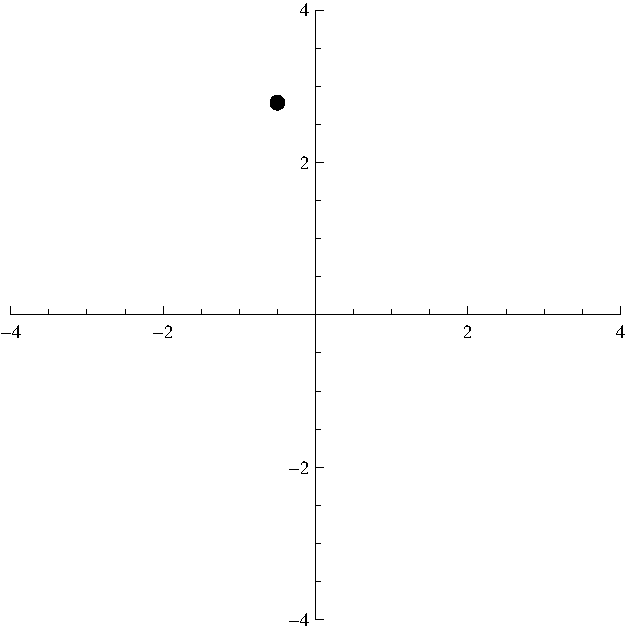
\includegraphics[width=3in]{../graphics/CmplxPlane1.pdf}
\]
Using the distance formula, we see:
\[
\sqrt{\left( \frac{-1}{2} \right)^2 + \left(\frac{31}{2}\right)^2} = 2\sqrt{2}
\]
Hence we can plot the point $\left(\frac{-1}{4\sqrt{2}}, \frac{31}{4\sqrt{2}}\right)$ on the unit circle:
\[
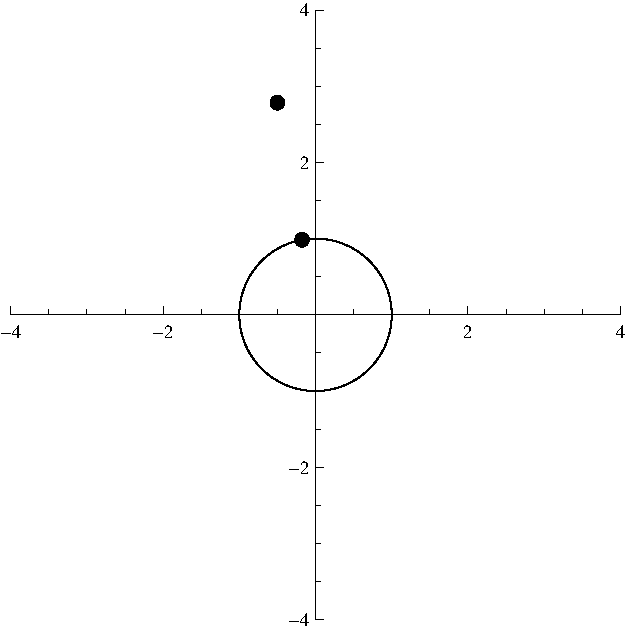
\includegraphics[width=3in]{../graphics/CmplxPlane2.pdf}
\]
Since multiplication of complex numbers lying on the unit circle in the
complex plane is simply rotation, the cube-root of $\frac{-1}{2} +
\frac{31}{2} i$ is:
\[
\left(\sqrt[3]{2\sqrt{2}}\right)\cos\left(\arcsin\left(\frac{31}{4\sqrt{2}}\right)/3\right) + i \left(\sqrt[3]{2\sqrt{2}}\right) \sin\left( \arcsin\left(\frac{31}{4\sqrt{2}}\right)/3\right)
\]
Gosh, that's a mess, plotted on the complex plane, it looks like the black point below:
\[
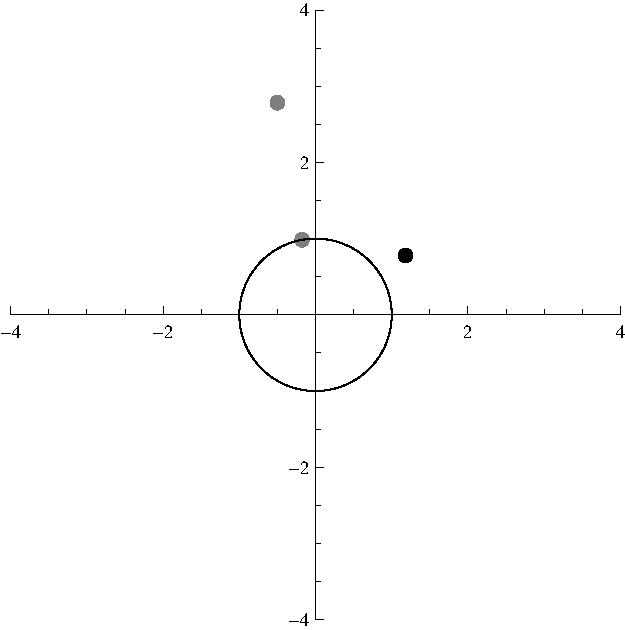
\includegraphics[width=3in]{../graphics/CmplxPlane3.pdf}
\]

Now we'll compute the cube-root of: 
\begin{align*}
\frac{8}{\frac{1}{2}(-1+\sqrt{-31})} = \frac{-1}{2} + \frac{-\sqrt{31}}{2} i 
\end{align*}
If we plot this in the complex plane, we get:
\[
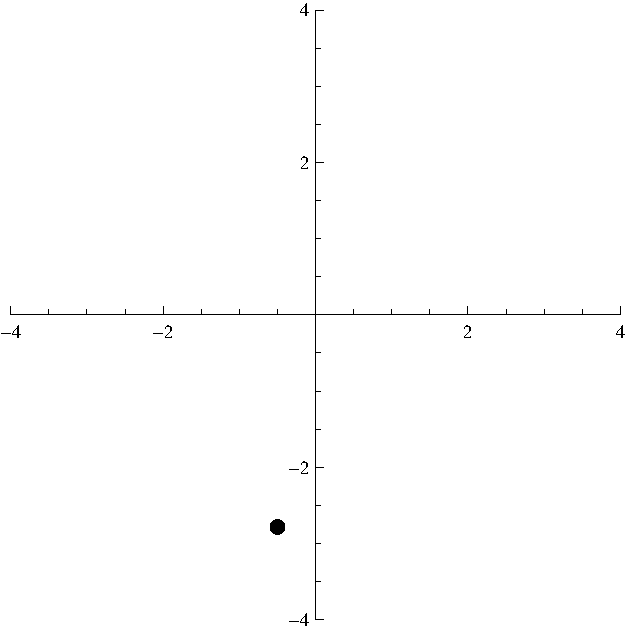
\includegraphics[width=3in]{../graphics/CmplxPlane4.pdf}
\]
Again, using the distance formula, we see:
\[
\sqrt{\left( \frac{-1}{2} \right)^2 + \left(\frac{31}{2}\right)^2} = 2\sqrt{2}
\]
Hence we can plot the point $\left(\frac{-1}{2}, \frac{-\sqrt{31}}{2} \right)$ on the unit circle:
\[
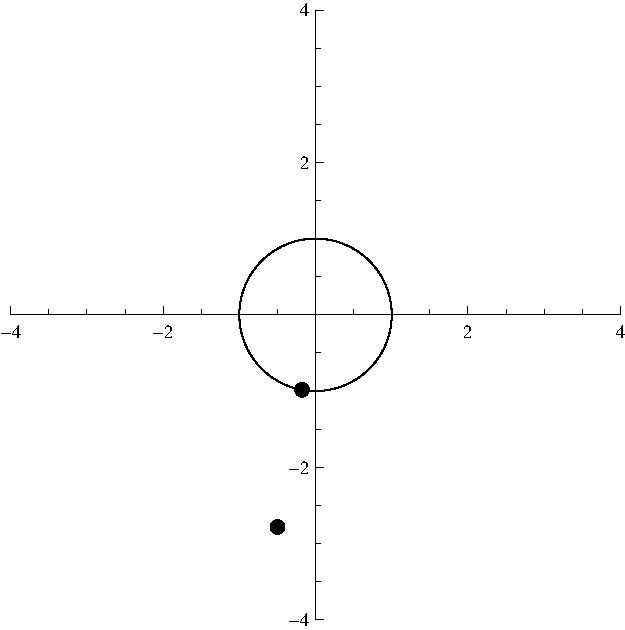
\includegraphics[width=3in]{../graphics/CmplxPlane5.pdf}
\]
Since multiplication of complex numbers lying on the unit circle in the
complex plane is simply rotation, the cube-root of $\frac{-1}{2} + \frac{-\sqrt{31}}{2} i $ is:
\[
\left(\sqrt[3]{2\sqrt{2}}\right)\cos\left(\arcsin\left(\frac{31}{4\sqrt{2}}\right)/3\right) - i \left(\sqrt[3]{2\sqrt{2}}\right) \sin\left( \arcsin\left(\frac{31}{4\sqrt{2}}\right)/3\right)
\]
Plotted on the complex plane, it looks like the black point below:
\[
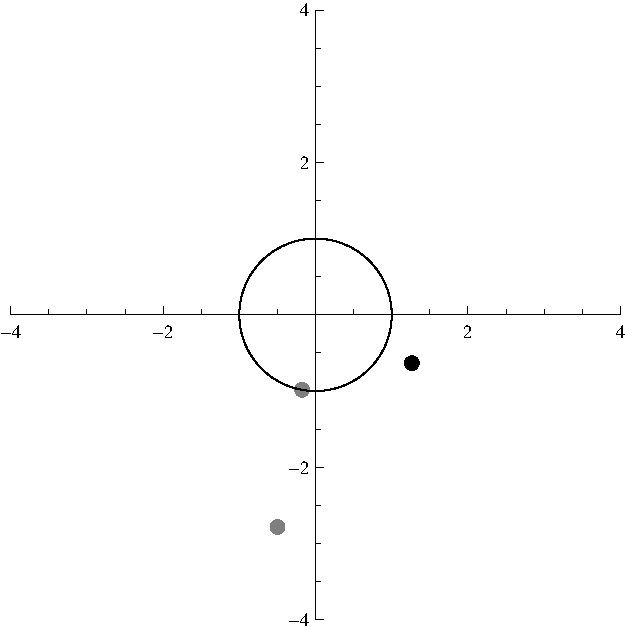
\includegraphics[width=3in]{../graphics/CmplxPlane6.pdf}
\]
Putting all of this together, we find:
\[
\sqrt[3]{\frac{-1+\sqrt{-31}}{2}} + \frac{2}{\sqrt[3]{\frac{1}{2}(-1+\sqrt{-31})}} = \left(2\sqrt[3]{2\sqrt{2}}\right)\cos\left(\arcsin\left(\frac{31}{4\sqrt{2}}\right)/3\right)
\]
A messy, but real, number. 


\newpage
\section{Tic-Tac-D'oh}

In the 17th and 18th centuries, finally mathematics was coming into
its own.  The codification of algebra, the introduction of the complex
numbers, the discovery of the calculus, all these formed the analogy
in their day of the introduction of the personal computer and the
Internet in modern times.  There was, if you will, an explosion of
mathematics (although among a very small community---unlike the recent
technological revolution).

The sense was that mathematics was this huge new tool that could be
applied to understand many, many things, from the movement of the
planets to the workings of business and industry.  And it wasn't long
before it was applied to the ancient human activity of gambling.  The
key was knowing more than your opponent about how the game would come
out.  Let's do an experiment with the game tic-tac-toe:

\begin{prob}
Consider the following set-up:
\[
\textsf{\begin{tabular}{c|c|c}
o & & x \\ \hline
x & x & o\\ \hline
o &   & 
\end{tabular}}
\]
It is currently \textsf{x}'s turn. What is the probablity
that \textsf{x} wins assuming that the rest of the moves are random?
\end{prob}


\begin{prob}
Consider the following set-up:
\[
\textsf{\begin{tabular}{c|c|c}
  & &  \\ \hline
o & x & \\ \hline
 &   & 
\end{tabular}}
\]
It is currently \textsf{x}'s turn. What is the probablity
that \textsf{x} wins in the next three moves assuming that the rest of
the moves are random?
% three solns count boards/count games/prob
% 15/7C2*5C1  or 30/7*6*5 or 6/7 * 5/6 * 1/4
\end{prob}



\newpage
\section{Bertrand's Paradox}

In this activity we are going to investigate the following question:

\begin{quote}
Given a circle, find the probability that a chord chosen at random is longer than the side of an inscribed equilateral triangle. 
\end{quote}

\paragraph{Method 1: Random Endpoints}

\begin{prob}
We want to define our chord via ``random endpoints.'' Explain why,
without loss of generality, we may assume that one of the endpoints is
on the vertex of the triangle.
\end{prob}

\begin{prob}
Draw a picture of the situation and use the arcs of the circle defined
by the triangle to help you determine the probability in question.
\end{prob}




\paragraph{Method 2: Random Radius}

\begin{prob}
We want to define our chord via a random point on a ``random radius.''
Explain why, without loss of generality, we may assume that any chord
is a random point on some radius of the circle.
\end{prob}

\begin{prob}
Draw a picture of the situation and use the length of the radius (in
relationship to the inscribed triangle) to help you determine the
probability in question.
\end{prob}


\paragraph{Method 3: Random Midpoint}

\begin{prob}
We want to define our chord via its midpoint. Explain why a midpoint
will (almost!) always determine a unique chord of a circle. When does
it fail? 
\end{prob}

\begin{prob}
Give a compass and straightedge construction for a chord given its
midpoint.
\end{prob}

\begin{prob}
Draw a picture of the situation along with the incircle of the
equilateral triangle to help you determine the probability in
question.
\end{prob}



\paragraph{Conclusion?!}

\begin{prob}
What did you find? How do we resolve the paradox?
\end{prob}


\newpage
\section{Tenths are Best}

Again in the 17th and 18th centuries, the algebra of the number system
was being established.  Numbers were associated to lengths, areas,
weights, etc., so that putting things together corresponded to adding
their associated numbers.

\begin{prob}
Give three examples of assigning a number to measure the size or shape
or position of a geometric or physical object so that putting the
objects together corresponds to adding the numbers.
\end{prob}


\begin{prob}
Give three examples of assigning a number to measure the size or shape
or position of a geometric or physical object so that putting the
objects together does \textit{not} correspond to adding the numbers.
\end{prob}

\begin{prob}
One example of the first problem is to assign a number to a line
segment (called its length).  
\begin{enumerate}
\item I want my system to be such that, by telling the number to someone half-way round the world, they will be able to make a line segment of the same length, that is, a line segment congruent to mine.  What do I need to do to make such an
assignment?
\item If I want to have a number for every possible line
segment, what kind of a number system will need to have?  Is the
system of rational numbers enough? That is, can you always construct a
segment whose length is not a fraction?  Why or why not?
\end{enumerate}
\end{prob}

\begin{prob}
The previous discussion led us to the decimal number system.  Decimals can be finite or infinite.
\begin{enumerate}
\item Describe how to add two infinite decimals.
\item Describe how to multiply 
\[
(0.111111\dots)\cdot (0.333333\dots)
\]
\item Describe how to multiply any two (infinite) decimals.
\end{enumerate}
\end{prob}


\begin{prob}
What is the relationship between $0.999999\dots$ and $1$? Can you
explain this?
\end{prob}


%\newpage
\section{Aye, Me Parrot Concurs}


Ahoy ye mateys! Imagine you be a 17th century pirate, and you have
three systems o'measurement:
\begin{enumerate}
\item An \textit{ar} for length.
\item An \textit{arr} for width.
\item An \textit{arrr} for depth. 
\end{enumerate}
Howe'er, thin's be not quite as simple as they seem.

\begin{prob}
Aye, my sunken ship had a rectangular deck, with a perimeter o'34 ars.
Its hull be $12$ arrrs deep for a might storage hold o'180 ars.
\end{prob}


\begin{prob}
MORE
\end{prob}


Ahoy ye mateys! Imagine you be a 17th century pirate, and you have
three systems o'measurement:
\begin{enumerate}
\item An \textit{ar} for length.
\item An \textit{arr} for area.
\item An \textit{arrr} for volume. 
\end{enumerate}
Howe'er, thin's be not quite as simple as they seem.

\begin{prob}
Aye, my ship be a rectangular deck, with a perimeter o'30 ars.
But it
\end{prob}




\newpage
\section{Whose Intimidating Who Now?}

In this activity, we'll investigate problems related to length, area,
and volume. To start, let me tell you a bit about myself. I'm about
$6'$ tall and I weigh about 160 pounds.

\begin{prob}
Imagine if you will, that one day I ``divide by zero'' and I am
fantastically made 100 times taller. Let's call this bigger
me \textit{monster-me.}
\begin{enumerate}
\item How tall is monster-me?
\item Relative to my eyeball, how much surface area does monster-me's eyeball have?
\item How much does monster-me weigh?
\end{enumerate}
\end{prob}


\begin{prob}
While you are probably imagining me as some sort of ``car-eating
monster,'' the reality is much different. I claim that monster-me
would have a hard time moving.  Can you explain why this is true?
\end{prob}

\begin{prob}
I also claim that monster-me would suffocate.  Can you explain why
this is true? Hint: How do lungs work? How does oxygen get to the
brain? How much blood would the monster-me have?
\end{prob}



\begin{prob}
Now imagine if you will, that one day I ``divide by infinity'' and I
am fantastically made 100 times smaller. Let's call this smaller me
\textit{mini-me.}
\begin{enumerate}
\item How tall is mini-me?
\item Relative to my eyeball, about how much surface area does mini-me's eyeball have?
\item How much does mini-me weigh?
\end{enumerate}
\end{prob}


\begin{prob}
I claim that mini-me would be able to fall from a great (relative)
height and be just fine.  Can you explain why this is true?
\end{prob}



\begin{prob}
When I was little, I used to want to fold a giant paper airplane and
actually fly around in it. Would this work? Why or why not?
\end{prob}





\newpage
\section{Diophantus---Fermat---Wiles}

Long before the invention of algebra, the Greek mathematician
constructed and solved riddles with whole numbers, several of which
are described in today's sketch.  Fermat had algebra at his disposal
and so was so taken with the number-riddles of Diophantus that he
recorded (and solved) many of them as equations where the solution
numbers should all be whole numbers (integers).  These have come to be
known as Diophantine equations.

\begin{prob}
One problem was to give all solutions to the Diophantine equation
\[
X^2 + Y^2 = Z^2
\]
remembering that $X$, $Y$, and $Z$ all have to be integers.
Diophantus would have asked ``Make a list of all the square numbers
that are the sum of two square numbers.''  Explain why this is the
same problem as solving 
\[
x^2 + y^2 = 1
\]
where $x$ and $y$ are rational numbers.
\end{prob}


\begin{prob}
In the plane below, draw the real-number solution set of $(x,y)$ so
that $x^2 + y^2 = 1$.
\begin{enumerate}
\item Find one rational-number solution $C = (x,y)$ to the equation such that neither $x$ nor $y$ is $0$.  Plot your solution $C$ in the plane below.
\item Draw the line through your solution and the solution $A = (0,1)$.  Mark the point $B$ at which your line crosses the $x$-axis.
\item Find the $x$-coordinate of $B$.  Is it a rational number?  Why or why not?
\end{enumerate}
\[
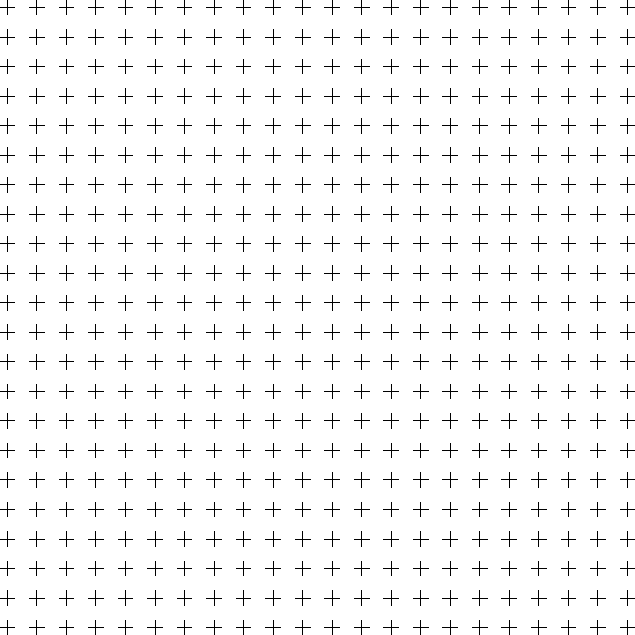
\includegraphics{../graphics/complexPlane.pdf}
\]
\end{prob}

\begin{prob}
Now on the grid below,
\begin{enumerate}
\item Draw the real-number solution set $x^2+y^2 = 1$, and mark the point $A' = (0,1)$.
\item Mark any point $B' = (r,0)$ inside the circle on the $x$-axis such that $r$ is a rational number.
\item Draw the line through $A'$ and $B'$.
\item Find the coordinates of the other point $C'$ at which your line cuts the solution set $x^2+y^2 =1$.  Are they rational numbers?  Why or why not?
\end{enumerate}
\[
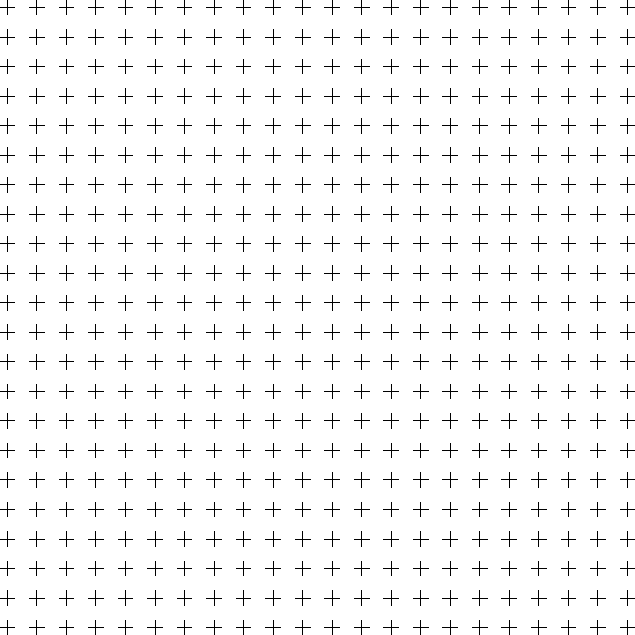
\includegraphics{../graphics/complexPlane.pdf}
\]
\end{prob}

\begin{prob}
Turn your solution $C'$ in the problem above into an integer solution
to the equation $X^2 + Y^2 = Z^2$.
\end{prob}



\newpage
\section{Cantor Can!}


It took until the 1700's to get algebra and number systems in place in
a workable way.  But there was still trouble understanding what
infinity was.  Was the set of counting numbers really infinite, or was
it only as big as the highest number that anyone had ever counted, or
as big as the number of atoms in the universe, or\dots?  But even if the
set of counting numbers was infinite, then the set of real numbers was
also infinite.  But then again, were they the same infinity?  Some
math grad student in Germany around 1850 shocked the math world by
saying `no.'


\begin{prob}
Here is a table of rational numbers:
\[
\begin{array}{|c|c|c|c|c|c|c|c|c|c|c|c|c|}\hline\bigstrut
\cdots & -5 & -4 & -3 & -2 & -1 & 0 & 1 & 2 & 3 & 4 & 5 & \cdots\\\hline\bigstrut
\cdots &\frac{-5}{2} & & \frac{-3}{2} &  & \frac{-1}{2} &   & \frac{1}{2} &  & \frac{3}{2} &  & \frac{5}{2} & \cdots\\\hline\bigstrut
\cdots & \frac{-5}{3} & \frac{-4}{3} & & \frac{-2}{3} & \frac{-1}{3} & & \frac{1}{3} & \frac{2}{3} & & \frac{4}{3} & \frac{5}{3} & \cdots\\\hline\bigstrut
\cdots & \frac{-5}{4} & & \frac{-3}{4} & & \frac{-1}{4} & & \frac{1}{4} & & \frac{3}{4} & & \frac{5}{4} & \cdots\\\hline\bigstrut
\cdots &  & \frac{-4}{5} & \frac{-3}{5} & \frac{-2}{5} & \frac{-1}{5} & & \frac{1}{5} & \frac{2}{5} & \frac{3}{5} & \frac{4}{5} &  & \cdots\\\hline\bigstrut
       & \vdots & \vdots & \vdots & \vdots & \vdots & \vdots & \vdots & \vdots & \vdots & \vdots & \vdots & \\\hline
\end{array}
\]
\begin{enumerate}
\item What does the 12th row of the table look like? 
\item Name three different rational numbers. Will they (eventually) appear on the table?
\item Will every rational number eventually appear in the table above?
\item Can you figure out how to ``enumerate'' the rationals?
\end{enumerate}
\end{prob}


\begin{prob}
The question: Are the set of counting numbers and the set of real
numbers between $0$ and $1$ the same size?

Cantor's answer: Suppose they were, then you could make a one-to-one,
onto match-up:
\begin{align*}
1 &:0\,.\,2\,2\,3\,4\,3\,7\,9\,8\,7\,8\,4\,\dots\\
2 &:0\,.\,8\,5\,9\,8\,4\,7\,5\,9\,3\,4\,8\,\dots\\
3 &:0\,.\,1\,1\,2\,9\,0\,2\,9\,3\,9\,8\,0\,\dots\\
4 &:0\,.\,0\,3\,4\,3\,2\,3\,4\,0\,5\,6\,3\,\dots\\
5 &:0\,.\,9\,3\,9\,2\,8\,4\,9\,8\,2\,3\,9\,\dots\\
6 &:0\,.\,7\,9\,7\,8\,8\,9\,3\,7\,8\,3\,3\,\dots\\
  &\;\vdots
\end{align*}
So, you think you did it, eh?  I will find a real number between zero
and one that is not on your list.  How will I do it?
\end{prob}

\begin{prob}
Explain why the same argument does \textit{not} show that the
rationals cannot be enumerated.
\end{prob}


\newpage
\section{Can You Repeat the Question?}


Explain why the following ``joke'' is ``funny.''
\begin{quote}
If you choose an answer to this question at random, what is the chance you will be correct?
\begin{enumerate}
\item 25\%
\item 50\%
\item 75\%
\item 25\%
\end{enumerate}
\end{quote}




\newpage
\section{The Applied Side---Stat!}

While Cantor was doing very abstract and pure mathematics in Germany,
statistics was making its first appearance as a mathematical subject
in England.  In this activity, we are going to investigate the \textit{mean}, \textit{median}, and \textit{mode} of a set of data. 


\begin{prob}
Explain what is meant by the mean, median, and mode of a set.
\end{prob}

\begin{prob}
Give a set of data consisting of $6$ values (not all equal!) such that
the mean, median, and mode are all equal. Plot your data in some
reasonable way.
\end{prob}

\begin{prob}
Give a set of data consisting of $6$ values such that the mean is
larger than both the median and mode which are equal. Plot your data in
some reasonable way.
\end{prob}


\begin{prob}
Give a set of data consisting of $6$ values such that the mode is
larger than both the mean and median. Plot your data in some
reasonable way.
\end{prob}

\paragraph{Simpson's Paradox}


In the 1970's a scandal arose at the University of California,
Berkley. There was a distinct gender bias against women in the number
of graduate students admitted among the 6 largest departments:
\[
\begin{tabular}{|c||c|c|} \hline
 & Applicants & Admitted \\ \hline\hline
Men & 2590 & 46\% \\ \hline
Women & 1835 & 30\% \\ \hline
\end{tabular}
\]
Data from individual departments was collected for further investigation:
\[
\begin{tabular}{|c||c|c||c|c|} \hline
\multirow{2}{*}{Department} & \multicolumn{2}{c||}{Men} & \multicolumn{2}{c|}{Women}  \\\cline{2-5}
 & Applicants & Admitted & Applicants & Admitted \\\hline\hline
A & 825 & 62\% & 108 & 82\%\\ \hline
B & 560 & 63\% & 25 & 68\% \\ \hline
C & 325 & 37\% & 593 & 34\% \\ \hline
D & 417 & 33\% & 375 & 35\% \\ \hline
E & 191 & 28\% & 393 & 24\% \\ \hline
F & 272 & 6\% & 341 & 7\% \\ \hline
\end{tabular}
\]

\begin{prob}
Examine this data critically. What seems to be the case? Does this
jive with your intuition? What is actually happening? Can you explain
when this will happen?
\end{prob}


%Perhaps it is not surprising that a cousin of Charles
%Darwin was involve, inventing correlation and regression as
%statistical methods to study the evolution of the human species.

%As an example of what correlation means, suppose there were four sets
%of twin females that were split up at birth with one twin living her
%life in the U.S. and the other twin living her life in England.
%Suppose the average adult height of a female in the U.S.\ is 5'4'' with
%a standard deviation of 2'' and the average adult height of a female in
%England is 5'6'' with a standard deviation of 3''.
%\[
%\begin{tabular}{|l||l|l|}\hline
%Twin set & U.S. & U.K. \\ \hline\hline
%1 & 5'6'' & 5'6'' \\\hline
%2 & 5'5'' & 5'4'' \\\hline
%3 & 5'6'' & 5'8'' \\\hline
%4 & 4'11'' & 5'6'' \\\hline
%\end{tabular}
%\]



%\begin{prob}
%Compute the correlation coefficient of this paired (twin) data using
%either formula for $r$ below.  

%Recall two methods of computing the \textit{sample correlation
%coefficient}, commonly denoted $r$:
%\[
%r = \frac{\sum_{i=1}^n(X_i-\bar{X})(Y_i-\bar{Y})}{\sqrt{\sum_{i=1}^n(X_i-\bar{X%})^2}\sqrt{\sum_{i=1}^n(Y_i-\bar{Y})^2}}
%\]
%An equivalent expression gives the correlation coefficient as the mean
%of the products of the standard scores.  Based on a sample of paired
%data $(X_i, Y_i)$, the sample correlation coefficient is:
%\[
%r = \frac{1}{n-1}\sum_{i=1}^n \left(\frac{X_i-\bar{X}}{\sigma_X} \right)\left(\frac{Y_i-\bar{Y}}{\sigma_Y} \right)
%\]
%\end{prob}

%\begin{prob}
%Figure out a single change in the data that makes the correlation
%coefficient bigger.
%\end{prob}



%Recall that Pearson's correlation coefficient between two variables is
%defined as the covariance of the two variables divided by the product
%of their standard deviations:
%\[
%\rho_{X,Y} = \frac{\mathrm{cov}(X,Y)}{\sigma_X\sigma_Y} = \frac{E[(X-\mu_X)(Y-\%mu_Y)]}{\sigma_X\sigma_Y}
%\]
%The above formula defines the \textit{population correlation
%coefficient}, commonly represented by the Greek letter $\rho$
%(rho). Substituting estimates of the covariances and variances based
%on a sample gives the
%\textit{sample correlation coefficient}, commonly denoted $r$:


%\newpage
\section{Voting Woes}	


In this activity, we are going to investigate the condrums that arise
when voting. With this in mind, I think it might be fitting to include
one of my favorite quotes:

\begin{quote}
If people do not believe that mathematics is simple, it is only because they do not realize how complicated life is.  

\hfill---John von Neumann
\end{quote}

With that said, let's go! There are lots of different voting
systems---here we describe three of them:

\paragraph{Plurality Voting:} Count the votes. The person with the most votes wins.
\paragraph{Vote For Two:} Everybody has two votes. Count the votes. The person with the most votes wins.
\paragraph{Borda Count:} Rank your candidates. Sum the ranks. The person with the \textbf{lowest} sum wins.



\begin{prob}
Cookie Monster, Big Bird, Grover
\end{prob}

\[
\begin{tabular}{|c|c|c|c|}\hline
Votes & First Preference & Second Preference & Third Preference & \\ \hline\hline
10    &  Cookie Monster  & 

\end{tabular}
\]

\begin{prob}

\end{prob}


Condorcet's Paradox



\newpage
\section{\sout{Deci}mals, \textit{Bi}-mals}


We use the decimal system to denote real numbers, but computers
don't. They use a ``sophisticated'' elaboration, \textit{bi-mals}.
That is, they would denote the number $101$ as:
\[
1\cdot 2^6 + 1\cdot 2^5 + 0 \cdot 2^4 + 0\cdot 2^3 + 1 \cdot 2^2 + 0 \cdot 2^1 + 1\cdot 2^0 = \text{``1100101''}
\]
Let's pretend like we are computers and work exclusively with bi-mals!

\begin{prob}
Calculate $1100+110$ by hand.
\end{prob}

\begin{prob}
Calculate $1100\cdot 110$ by hand.
\end{prob}


\begin{prob}
Calculate $1100101^{10}$ by hand. Remember that the exponent is a
bi-mal number too!
\end{prob}


Computers use the ``bi-mal point'' to write all real numbers in
bi-mal.  For example:
\[
1\cdot 2^2 + 1\cdot 2^1 + 0 \cdot 2^0 + 0\cdot 2^{-1} + 1 \cdot 2^{-2} + 0 \cdot 2^{-3} + 1\cdot 2^{-4} = \text{``110.0101''}
\]


\begin{prob}
Do the following bi-mal long division problem
\[
11\,\begin{array}[b]{@{}r@{}r} 
 & \\ 
\cline{1-1}
\big)\begin{array}[t]{@{}l@{}} 1100101 
\end{array}
\end{array}
\]
\end{prob}

\begin{prob} Express $\dfrac{1}{7}$ as a bi-mal. 
\end{prob}

\begin{prob} Which bi-mal fractions will terminate? Which will repeat?
\end{prob}

\begin{prob}
Calculate $110.0101^{10}$ by hand. 
\end{prob}




\newpage
\section{Roll Play This}

Long before the \textit{World of Warcraft}, but not as long ago
as \textit{The Lord of the Rings}, there was a game
called \textit{Dungeons\&Dragons}. In this game you played a
``character'' with abilities such as strength, dexterity, and so
on. You computed these abilities by rolling a 6-sided die three times
and adding the numbers up (denoted 3d6). To give you a little feel for this, suppose
you were making your own character, and you were finding their
``Math-Class'' ability. Fill out the form below:
\[
\fbox{\begin{minipage}{60ex}
\vspace{.5cm}
Name:$\underset{\text{(make up a creative name for yourself)}}{\protect\rule[-2pt]{3in}{.5pt}}$\hfill\\
Math-Class Ability: $\underset{\text{(Roll 3d6)}}{\fbox{\rule[0mm]{0mm}{3ex}\hspace{3ex}}}$ 
\end{minipage}}
\]


Let's see how your character does in a made-up math class: (roll a
20-sided die 4 times and count how many times it rolls \textbf{below}
your ``Math-Class'' ability.)
\begin{itemize}
\item[4:] A congratulations!
\item[3:] B nice!
\item[2:] C no worries!
\item[1:] D is for diploma!
\item[0:] E umm\dots
\end{itemize}

As you can see, the game was thrilling. My question is this: Why do
they use the sum of rolling a 6-sided die 3 times to determine
the abilities? Let's see if we can figure this out.

\begin{prob}
Roll a 3d6 5 times and write down what you get. Demand that your
results are shared with the class and see what you get.
\end{prob}


\begin{prob}
Compute the \textit{relative frequency} of obtaining different results
for ``math ability.''
\end{prob}


\begin{prob}
Compute the \textit{probability} of obtaining different results
for ``math ability.''
\end{prob}

\begin{prob}
Can you explain why 3d6 was chosen to determine ability scores in the
game?
\end{prob}




\newpage
\section{It's How You Play The Game}

Let's play a game! Here is how it will work: Taking turns, each of you
will pick a square on the chart below to be ``yours.'' Continue until
every square is chosen.
\[
\begin{array}{|c|c|c|c|c|c|} \hline
1 & 2 & 3 & 4 & 5 & 6 \\ \hline
7 & 8 & 9 & 10 & 11 & 12 \\ \hline
\end{array}
\]
Then you will roll some dice. If your number comes up, you get a
point! First to $10$ points wins.


\begin{prob}
Play the game with a $12$-sided die. Does it matter which square you
chose? Explain your thoughts on this.
\end{prob}

\begin{prob}
Play the game with two $6$-sided dice, adding their values
together. Does it matter which square you chose? Explain your thoughts
on this.
\end{prob}


\begin{prob}
Play the game with three  $4$-sided dice, adding their values
together. Does it matter which square you chose? Explain your thoughts
on this.
\end{prob}


\begin{prob}
Compute the probability of rolling different squares with a 12-sided
die, two 6-sided dice, and three 4-sided dice. Make three charts to
help you out. What do you notice?
\end{prob}

Now let's change the rules of the game. In this game, you get the number of points of the square you are on. So if you choose ``square 3'' and you roll a 3, you get 3 points! First to $80$ wins!

\begin{prob}
Now which is the best square to choose if you are playing with:
\begin{itemize}
\item One 12-sided die?
\item Two 6-sided dice?
\item Three 4-sided dice?
\end{itemize}
\end{prob}

Note, if you enjoyed this game, check out \textit{Settlers of Catan}.




\end{document}
